\subsection{Présentation de WORDLE}
\tabto{1cm}Notre jeu est basé largement sur le jeu Wordle du New York Times. Le principe est d’essayer de deviner un mot secret en le moins de coups possible. Dans le jeu original le mot secret a cinq lettres, pour chaque tentative l’utilisateur doit essayer un mot qui existe dans le dictionnaire du jeu. En utilisant des couleurs différentes, le jeu donne des indices : si une des lettres du mot essayé est à la bonne place dans le mot secret, la lettre devient verte ; si elle est dans le mot mais mal placée elle devient jaune, sinon la lettre n’est pas dans le mot et reste grise. Le joueur a un maximum de 6 essais pour trouver le mot, et le jeu s’arrête lorsque le mot secret est trouvé ou bien si le joueur n’a plus de tentatives. Nous avons préservé les principes fondamentaux du jeu, mais nous avons donné au joueur la liberté de choisir la longueur du mot secret ainsi que le nombre de tentatives maximum.

\subsection{Présentation de l'application Web}
\subsection{Schéma de la base de données et modèle entité-association}
Notre base de données est constitué de 4 tables:
\begin{itemize}
    \item Une table User dont les colonnes sont : idUser qui est l’identifiant du joueur de type entier, un pseudo qui représente le nom du joueur de type str, un mot de passe de type str et une chaîne de caractère salt pour la sécurisation du compte utilisateur. La chaîne de caractères stockée dans la colonne mot\_de\_passe sera le haché de la concaténation du mot de passe et du salt.
    \item Une table Partie dont les colonnes sont : idPartie qui représente l’identifiant d’une partie de type int, idUser qui est une clé étrangère, les points d'expérience de type int qui représente les points gagnés lors d’une partie, le mot secret associé à la partie de type str, le nombre de coups mis par le joueur pour trouver le mot secret de type int, le nombre d’essais maximum de la partie de type int et la longueur des mots associé à la partie de type int.
    \item Une table AchievementDesc dont les colonnes sont: idSucces qui est l’identifiant de l’achievement et description la description associée (“gagner une partie en 2 coups”, “gagner 10 parties” etc\dots{}).
    \item Une table Achievements qui relie les tables AchievementDesc et partie dont les colonnes sont : idPartie clé étrangère et idSucces clé étrangère. Ces 2 clés forment la clé primaire de la table Achievements.
\end{itemize}

\begin{figure}[h!]
\centering
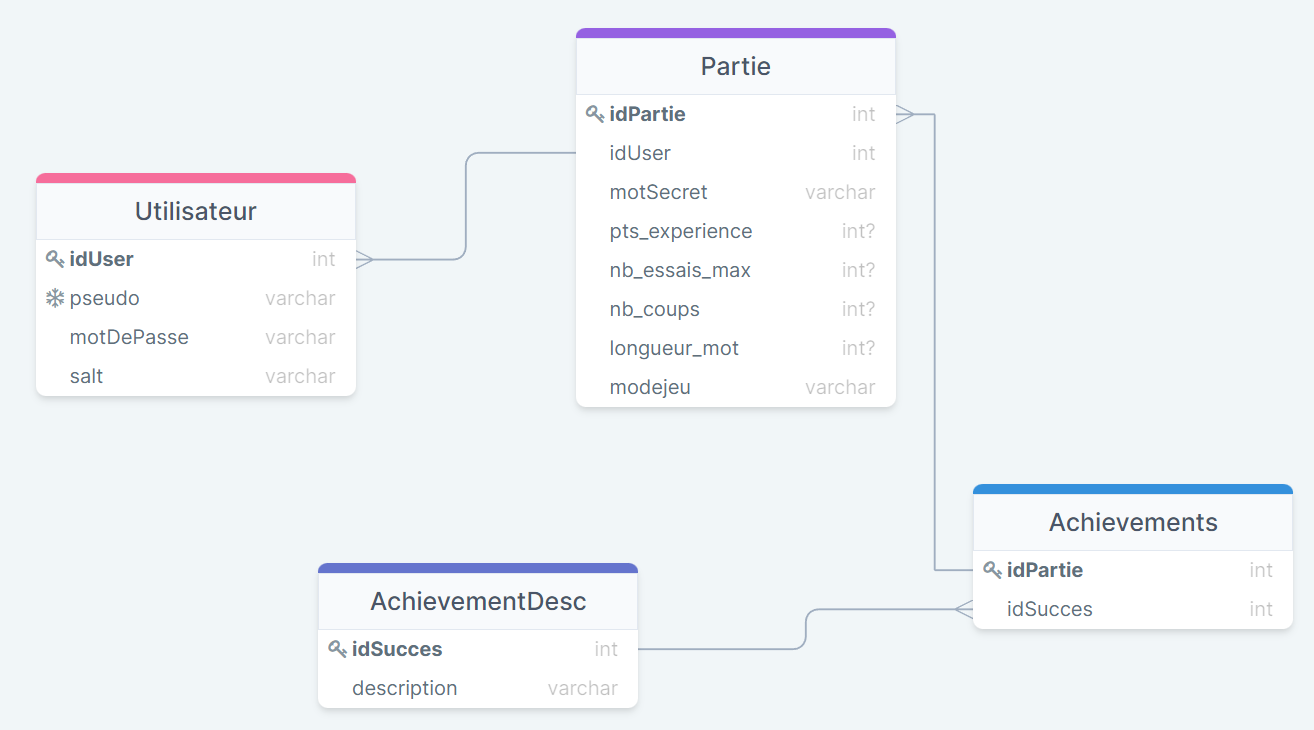
\includegraphics[width=12cm]{figures/bddfinale.PNG}
\caption{Schéma de la base de données de WORDLE}
\end{figure}

\break

\subsubsection{Agencement des pages HTML et des routes}
Le site sera composé de cinq pages HTML :
\begin{itemize}
    \item index.html, la page d’accueil et la page de jeu. Elle est la page centrale du site : depuis index.html, on peut se créer un compte, se connecter et consulter son profil une fois connecté. À noter que créer un compte n’est pas obligatoire pour jouer mais, dans ce cas, aucune partie ne sera enregistrée et aucun achievement ne sera délivré.
    \item register.html, où un joueur peut se créer un compte. Après avoir vérifié que le pseudo renseigné est disponible, les données sont enregistrées dans la table User.
    \item login.html, où le joueur peut se connecter. La connexion réussit si les informations d’authentification (pseudo et mot de passe) renseignées sont valides et échoue sinon.
    \item profile.html, où le joueur peut consulter les informations relatives à son profil. Ces informations sont l’historique des parties effectuées, les statistiques relatives à ces parties et les succès débloqués par le joueur.
    \item settings.html, où le joueur peut choisir le mode de jeu ainsi que la longueur du mot à deviner et le nombre maximum de tentatives autorisées.
\end{itemize}

Quant aux routes, elles seront organisées de la manière suivante :

\begin{figure}[h!]
\centering
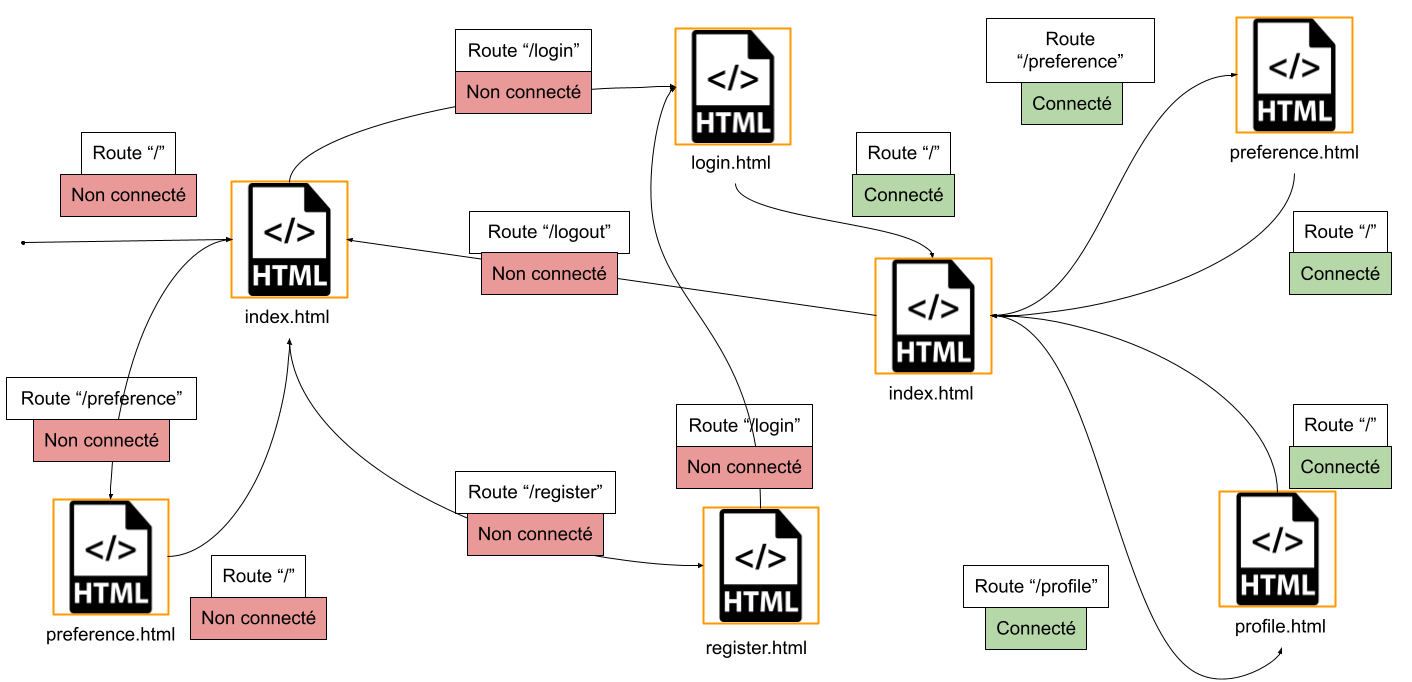
\includegraphics[width=12cm]{figures/schema_routes.png}
\caption{Organisation des routes de WORDLE}
\end{figure}

\subsubsection{Implémentation du jeu}
\textbf{Fonctionnement global} \\

\tabto{1cm}Notre jeu est constitué d’une grille dont les dimensions sont paramétrables par le joueur. Étant donné les paramètres, on crée en JavaScript une grille dont chaque case a un identifiant unique. A l’aide d’un gestionnaire d'événements de clavier, on récupère chaque lettre majuscule tapée par l’utilisateur et on l’insère dans chaque case de la gauche vers la droite jusqu’à ce qu’on atteigne la longueur du mot définie par l’utilisateur. L’utilisateur a également la possibilité d’effacer une lettre rentrée. Aussi, lorsqu’il tape “entrer” et que la longueur du mot entré est égale à celle choisie par l’utilisateur, il verra chaque case contenant chaque lettre se colorer selon la position de la lettre dans le mot secret. Il faut noter que le mot secret est choisi arbitrairement dans le dictionnaire et est caché dans une balise html.\\

\tabto{0cm}\textbf{Fin du jeu}\\

\tabto{1cm}Dans une liste, nous récupérons chaque lettre jusqu’à ce qu’on atteigne la longueur du mot secret. Cette liste est ajoutée dans une autre liste vide définie préalablement et à chaque fois que le mot ne correspond pas au mot secret, on réitère le processus.
Lorsqu’on atteint le nombre d’essais maximum ou lorsque le mot est trouvé, la partie se termine et un bouton “rejouer” s’affiche dans le cas où un utilisateur voudrait rejouer le jeu. 


\subsubsection{Maquette du site}
Voici le premier design du site :

\begin{figure}[h!]
\centering
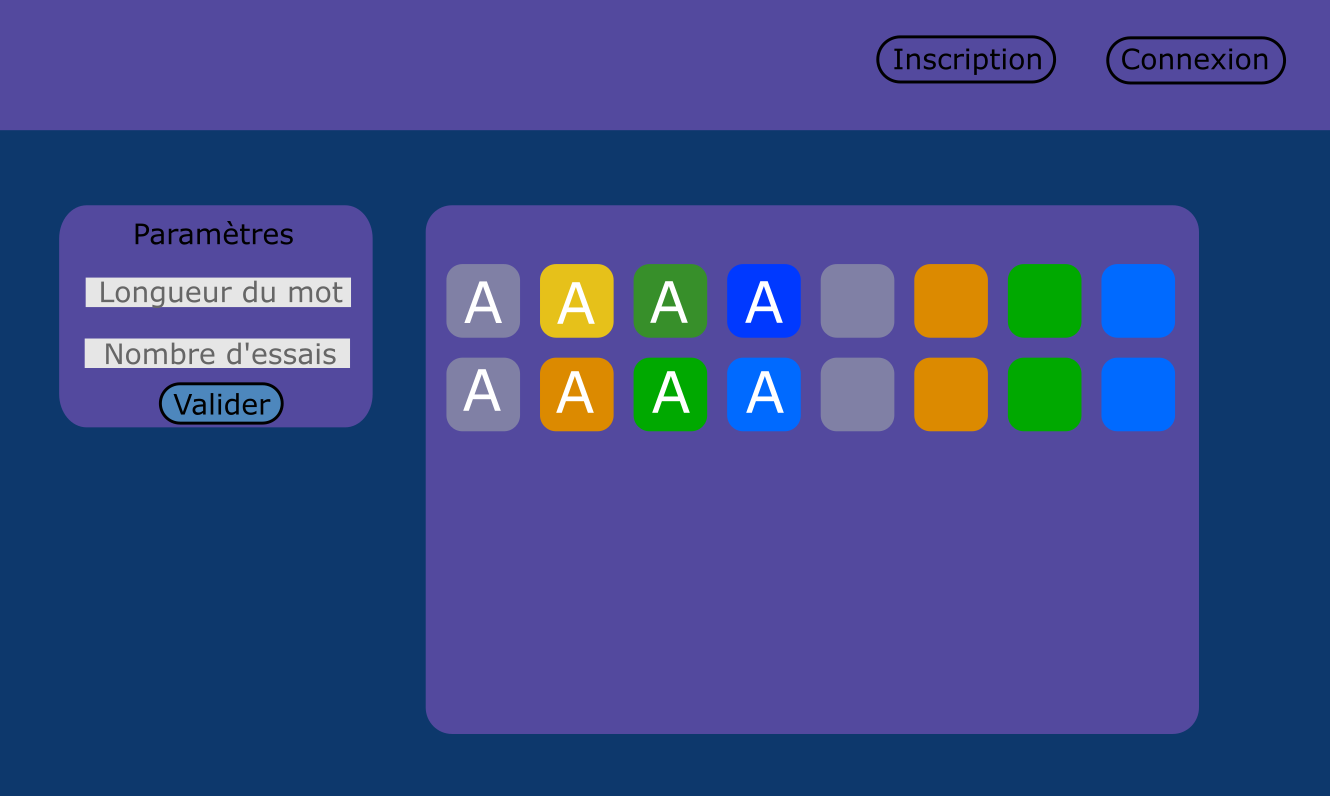
\includegraphics[width=12cm]{figures/wordle_sketch.PNG}
\caption{Première maquette de WORDLE}
\end{figure}
Ce design représente la page index.html lorsque le joueur est déconnecté. Le logo se situerait en haut à gauche. Les couleurs sont potentiellement sujettes à modification.

\subsubsection{Paramétrage du jeu et profil utilisateur}
\tabto{1cm}Le paramétrage du jeu, c’est-à-dire le choix du mode de jeu, de la longueur du mot à deviner ainsi que du nombre de tentatives autorisées est entièrement paramétrable par le joueur sur la page de jeu.

\tabto{1cm}Sur la page profile.html, chaque joueur aura accès à l’historique de ses parties (pour chaque partie, voir quel était le mot secret et si la partie a été gagnée ou non), ses statistiques de jeu (le nombre moyen de coups par partie, le pourcentage de victoire et son nombre de parties jouées) et aux achievements (succès) qu’il aura débloqué en jouant. Pour ce qui est des statistiques, elles seront déclinées en fonction de la longueur du mot : pour chaque longueur de mot différente, on aura un volet “nombre moyen de coups par partie” et un volet “pourcentage de victoire” en plus des statistiques globales.

\subsubsection{Solveur}

\tabto{1cm}Le solveur permet au joueur de penser a un mot que le solveur doit deviner en suivant les règles du jeu. Le solveur est codé exclusivement en langage C et utilise des structures de données les plus appropriées, à savoir une table de hachage permettant au solveur de trouver les mots rapidement. \\

\tabto{1cm}Au lancement du programme, le solveur explique au joueur comment jouer et le joueur répond dans le terminal. Le joueur donne des indices au solveur de la même façon que le jeu WORDLE donne des indices au joueur. Si le joueur veut arrêter le jeu, il met -1 dans le terminal, sinon il donne une chaîne de la même longueur que le mot avec des chiffres 0,1 et 2 : 2 représente une lettre bien placée, 1 représente une lettre correcte mal placée et 0 représente une lettre qui ne se trouve pas dans le mot. En fonction des réponses du joueur, le solveur retourne au joueur le mot le plus probable. Par exemple, si le mot recherché est ARBRE et que le solveur propose NAGER, le joueur est obligé de répondre avec ‘01011’.

\begin{figure}[h!]
\centering
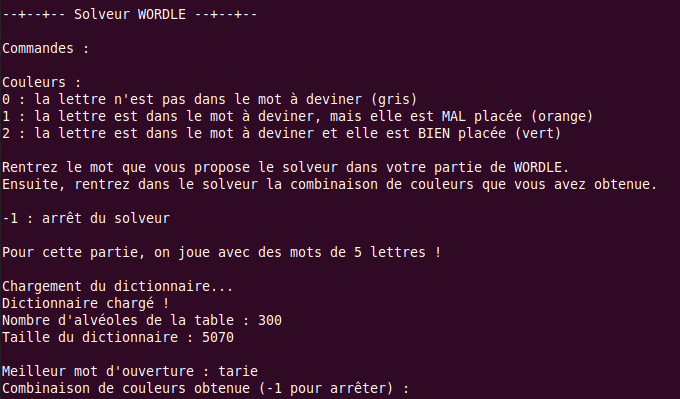
\includegraphics[width=12cm]{figures/avant.PNG}
\caption{Avant de jouer}
\end{figure}

\begin{figure}[h!]
\centering
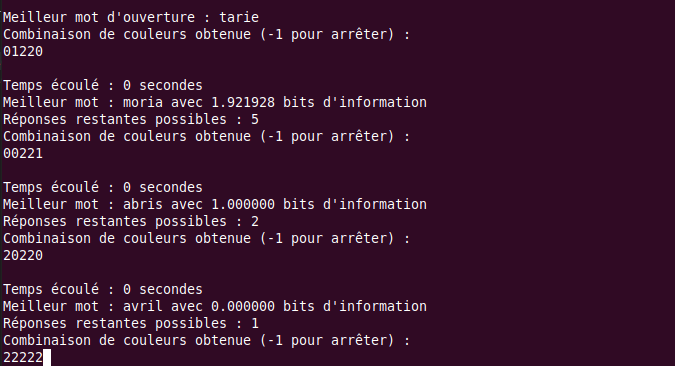
\includegraphics[width=12cm]{figures/solveur_gagne.PNG}
\caption{En jouant}
\end{figure}